\documentclass[12pt,a4paper]{article}
\usepackage[utf8]{inputenc}
\usepackage[T1]{fontenc}
\usepackage{geometry}
\usepackage{amsmath, amssymb}
\usepackage{booktabs}
\usepackage{listings}
\usepackage{xcolor}
\usepackage{hyperref}
\usepackage{parskip}

\geometry{margin=1in}

% ── Python Listing Style ──────────────────────────────────────────────────────
\definecolor{codebg}{RGB}{248,248,248}
\definecolor{codegreen}{rgb}{0,0.6,0}
\definecolor{codegray}{rgb}{0.5,0.5,0.5}
\definecolor{codeblue}{rgb}{0,0,0.8}
\definecolor{codeorange}{rgb}{0.8,0.4,0}

\lstdefinestyle{pythonstyle}{
    language=Python,
    backgroundcolor=\color{codebg},
    basicstyle=\ttfamily\footnotesize,
    keywordstyle=\color{codeblue}\bfseries,
    commentstyle=\color{codegreen}\itshape,
    stringstyle=\color{codeorange},
    numbers=left,
    numberstyle=\tiny\color{codegray},
    stepnumber=1,
    numbersep=8pt,
    tabsize=4,
    showstringspaces=false,
    breaklines=true,
    frame=single,
    captionpos=b,
    morekeywords={self, True, False, None, np, pd, plt, sns}
}
\lstset{style=pythonstyle}
% ─────────────────────────────────────────────────────────────────────────────

\title{\textbf{Dokumentasi Kode} \\ \large Replikasi Eksperimen Giudici et al. (2020) \\
\small \texttt{strategy\_comparison.ipynb}}
\author{Catatan Tesis}
\date{\today}

\begin{document}

\maketitle
\tableofcontents
\newpage

%=============================================================================
\section{Pendahuluan}
%=============================================================================
Dokumen ini merinci implementasi kode untuk membandingkan strategi \textit{Network Markowitz} terhadap berbagai baseline dalam ekosistem aset kripto. Eksperimen ini merupakan replikasi dari penelitian Giudici et al. (2020) berjudul \textit{"Network Models to Improve Automated Cryptocurrency Portfolio Management"}.

Strategi yang dibandingkan meliputi:
\begin{enumerate}
    \item \textbf{Equally Weighted (EW)}: Portofolio naif ($1/N$).
    \item \textbf{Classical Markowitz (CM)}: Optimasi Mean-Variance tradisional.
    \item \textbf{Glasso Markowitz (GM)}: Markowitz dengan regularisasi \textit{Graphical Lasso}.
    \item \textbf{Network Markowitz (NW)}: Integrasi \textit{Random Matrix Theory} (RMT) dan \textit{Minimum Spanning Tree} (MST).
    \item \textbf{Graph Diversification}: Strategi diversifikasi berbasis teori graf menggunakan \textit{Maximum Independent Set} (MIS).
\end{enumerate}

%=============================================================================
\section{Sel 1 -- Persiapan Library}
%=============================================================================
\begin{lstlisting}[caption={Import libraries dan konfigurasi visualisasi}]
import numpy as np
import pandas as pd
import matplotlib.pyplot as plt
import seaborn as sns
import networkx as nx
from scipy.optimize import minimize
from scipy.sparse.csgraph import minimum_spanning_tree
from scipy.linalg import eigh
from sklearn.covariance import GraphicalLassoCV
import warnings
warnings.filterwarnings('ignore')

plt.style.use('seaborn-v0_8-darkgrid')
sns.set_palette("husl")

print("Libraries imported successfully!")
\end{lstlisting}

%=============================================================================
\section{Sel 2 -- Memuat Data}
%=============================================================================
Memuat data return dan harga dari file Excel. Fokus utama adalah pada dataset return harian untuk 10 aset kripto utama dalam periode 14 September 2017 hingga 17 Oktober 2019.

\begin{lstlisting}[caption={Load dataset kripto}]
# Load data
excel_file = 'crypto_data_real.xlsx'
df_returns = pd.read_excel(excel_file, sheet_name='Returns', index_col=0)
df_prices = pd.read_excel(excel_file, sheet_name='Prices', index_col=0)

crypto_names = df_returns.columns.tolist()
n_assets = len(crypto_names)

print(f"Data loaded: {df_returns.shape[0]} days, {n_assets} assets")
print(f"Period: {df_returns.index[0]} to {df_returns.index[-1]}")
\end{lstlisting}

%=============================================================================
\section{Sel 3 -- Statistik Ringkasan (Summary Statistics)}
%=============================================================================
Bagian ini menghasilkan tabel statistik deskriptif untuk setiap aset kripto, mencakup Mean, Standar Deviasi, Kurtosis, dan Skewness sesuai dengan standar pelaporan dalam literatur keuangan (seperti Tabel 1 pada paper acuan).

\begin{lstlisting}[caption={Kalkulasi statistik deskriptif aset}]
# Create summary statistics table
summary_stats = pd.DataFrame({
    'Mean': df_returns.mean(),
    'Std': df_returns.std(),
    'Kurtosis': df_returns.kurt(),
    'Skewness': df_returns.skew()
})
print("TABLE 1 | Summary statistics.")
print(summary_stats.round(4))
\end{lstlisting}

%=============================================================================
\section{Sel 4 -- Visualisasi Harga Ternormalisasi (Figure 1 \& 2)}
%=============================================================================
Grafik di bawah ini mereplikasi "Normalized cryptocurrency price series" dengan mengatur harga awal setiap aset menjadi 100 pada tanggal 7 Januari 2018.

\begin{lstlisting}[caption={Dua set plot harga ternormalisasi}]
# --- Figure 1: BTC, ETH, USDT, BCH, LTC ---
assets_1  = ['BTC', 'ETH', 'USDT', 'BCH', 'LTC']
df_norm_1 = (df_prices.loc['2018-01-07':, assets_1] / df_prices.loc['2018-01-07', assets_1]) * 100
colors_1  = ['black', 'red', 'green', 'blue', 'cyan']

plt.figure(figsize=(12, 5))
for i, col in enumerate(df_norm_1.columns):
    plt.plot(df_norm_1.index, df_norm_1[col], label=col, color=colors_1[i])
plt.title('Figure 1 | Normalized Price Series I (BTC, ETH, USDT, BCH, LTC)')
plt.ylabel('Normalized Price (base=100)')
plt.legend(); plt.tight_layout(); plt.show()

# --- Figure 2: XRP, BNB, EOS, XLM, TRX ---
assets_2  = ['XRP', 'BNB', 'EOS', 'XLM', 'TRX']
df_norm_2 = (df_prices.loc['2018-01-07':, assets_2] / df_prices.loc['2018-01-07', assets_2]) * 100
colors_2  = ['magenta', 'gold', 'lightgrey', 'black', 'red']

plt.figure(figsize=(12, 5))
for i, col in enumerate(df_norm_2.columns):
    plt.plot(df_norm_2.index, df_norm_2[col], label=col, color=colors_2[i])
plt.title('Figure 2 | Normalized Price Series II (XRP, BNB, EOS, XLM, TRX)')
plt.ylabel('Normalized Price (base=100)')
plt.legend(); plt.tight_layout(); plt.show()
\end{lstlisting}

%=============================================================================
\section{Sel 5 -- Visualisasi Minimum Spanning Tree (Figure 3 \& 4)}
%=============================================================================
Kode ini mereplikasi Figure 3 dari paper acuan, yang menunjukkan struktur jaringan aset kripto selama periode gelembung spekulatif (September 2017 -- Januari 2018). MST membantu mengidentifikasi aset yang menjadi pusat (hub) dalam sistem.

\begin{lstlisting}[caption={Konstruksi dan Plot MST}]
# Filter periode Speculative Bubble
df_bubble = df_returns.loc['2017-09-14':'2018-01-31']

# Hitung Matriks Jarak (Distance Matrix)
corr_bubble = df_bubble.corr()
dist_bubble = np.sqrt(2 * (1 - corr_bubble))

# Bangun Graf MST menggunakan NetworkX
G = nx.from_pandas_adjacency(dist_bubble)
mst_bubble = nx.minimum_spanning_tree(G, weight='weight')

# Plotting MST
plt.figure(figsize=(10, 8))
pos = nx.spring_layout(mst_bubble, seed=42) # Penempatan node
nx.draw(mst_bubble, pos, with_labels=True, node_color='orange', 
        node_size=1500, edge_color='black', linewidths=1.5, font_size=10, font_weight='bold')

plt.title('Figure 3 | MST September 2017 - January 2018', fontsize=12)
plt.show()

# --- Figure 4 | MST June 2019 - October 2019 ---
df_stable = df_returns.loc['2019-06-01':'2019-10-17']
corr_stable = df_stable.corr()
dist_stable = np.sqrt(2 * (1 - corr_stable))

G2 = nx.from_pandas_adjacency(dist_stable)
mst_stable = nx.minimum_spanning_tree(G2, weight='weight')

plt.figure(figsize=(10, 8))
pos2 = nx.spring_layout(mst_stable, seed=42)
nx.draw(mst_stable, pos2, with_labels=True, node_color='orange', 
        node_size=1500, edge_color='black', linewidths=1.5, font_size=10, font_weight='bold')

plt.title('Figure 4 | MST June 2019 - October 2019', fontsize=12)
plt.show()
\end{lstlisting}

%=============================================================================
\section{Sel 6 -- Fungsi Pembantu (Helper Functions)}
%=============================================================================
Bagian ini mengimplementasikan algoritma RMT untuk penyaringan noise pada matriks korelasi, konstruksi MST untuk jarak aset, serta metrik risiko seperti VaR dan \textit{Rachev Ratio}.

\begin{lstlisting}[caption={Algoritma Network dan Metrik Risiko}]
def apply_rmt_filter(returns_data):
    """Filter noise dari matriks korelasi menggunakan Random Matrix Theory."""
    if isinstance(returns_data, pd.DataFrame):
        data = returns_data.values
    else:
        data = returns_data
    T, N = data.shape
    Q    = T / N
    C    = np.corrcoef(data.T)

    eigenvalues, eigenvectors = eigh(C)
    eigenvalues  = eigenvalues[::-1]
    eigenvectors = eigenvectors[:, ::-1]

    lambda_plus      = 1 + (1/Q) + 2*np.sqrt(1/Q)          # Marcenko-Pastur upper bound
    significant_mask = eigenvalues > lambda_plus
    Lambda_filtered  = np.diag(np.where(significant_mask, eigenvalues, 0))
    C_filtered       = eigenvectors @ Lambda_filtered @ eigenvectors.T
    return C_filtered

def build_mst(correlation_matrix):
    distance_matrix = np.sqrt(2 - 2*correlation_matrix)
    np.fill_diagonal(distance_matrix, 0)
    return distance_matrix

def compute_eigenvector_centrality(distance_matrix):
    adjacency = 1 / (distance_matrix + 1e-8)
    np.fill_diagonal(adjacency, 0)
    eigenvalues, eigenvectors = eigh(adjacency)
    principal_eigenvector = np.abs(eigenvectors[:, -1])
    centrality = principal_eigenvector / principal_eigenvector.sum()
    return centrality

def calculate_var(returns, confidence=0.95):
    return np.percentile(returns, (1-confidence)*100)

def calculate_rachev_ratio(returns, alpha=0.10):
    threshold_upper = np.percentile(returns, (1-alpha)*100)
    threshold_lower = np.percentile(returns, alpha*100)
    cvar_upper = returns[returns >= threshold_upper].mean()
    cvar_lower = abs(returns[returns <= threshold_lower].mean())
    return cvar_upper / cvar_lower if cvar_lower > 0 else 0

def calculate_max_drawdown(cumulative_returns):
    running_max = np.maximum.accumulate(cumulative_returns)
    drawdown = (cumulative_returns - running_max) / running_max
    return drawdown.min()

def get_assets_graph_diversify(returns_window, corr_threshold=0.4):
    """Mencari aset untuk diversifikasi menggunakan Maximum Independent Set (MIS)."""
    corr_mat = returns_window.corr()
    G = nx.Graph()
    assets = list(returns_window.mean().sort_values(ascending=False).index)
    G.add_nodes_from(assets)
    for i, a1 in enumerate(assets):
        for a2 in assets[i+1:]:
            if abs(corr_mat.loc[a1, a2]) > corr_threshold:
                G.add_edge(a1, a2)
    return list(nx.approximation.maximum_independent_set(G))

\textit{Refinement: RMT-filtered Graph Selection}
\begin{lstlisting}[caption={Seleksi Aset MIS dengan Filter Noise RMT}]
def get_assets_graph_diversify_rmt(returns_window, corr_threshold=0.4):
    """Mencari aset independen menggunakan korelasi yang sudah difilter RMT."""
    assets = returns_window.columns.tolist()
    corr_f = apply_rmt_filter(returns_window) # Hasil RMT berupa numpy array
    G = nx.Graph()
    G.add_nodes_from(assets)
    for i, a1 in enumerate(assets):
        for j, a2 in enumerate(assets):
            if i < j and abs(corr_f[i, j]) > corr_threshold:
                G.add_edge(a1, a2)
    return list(nx.approximation.maximum_independent_set(G))
\end{lstlisting}
\end{lstlisting}

%=============================================================================
\section{Sel \textit{New} -- Analisis Dinamika MST (Figure 5)}
%=============================================================================
Untuk memahami evolusi struktur jaringan aset kripto, dilakukan analisis \textit{rolling window} untuk menghitung ambang batas MST (\textit{max link distance}) dan koefisien \textit{residuality}.

\begin{lstlisting}[caption={Kalkulasi dinamika MST (Figure 5)}]
def calculate_rolling_mst_metrics(returns_df, window=120):
    """Hitung dinamika MST dengan rolling window."""
    dates         = returns_df.index[window:]
    max_links     = []
    residualities = []

    for i in range(window, len(returns_df)):
        window_data  = returns_df.iloc[i - window:i]
        corr_f       = apply_rmt_filter(window_data)
        mst_weights  = build_mst(corr_f)
        max_links.append(np.max(mst_weights))
        residualities.append(np.sum(mst_weights) / (returns_df.shape[1] - 1))

    return pd.DataFrame(
        {'Max Link': max_links, 'Residuality': residualities},
        index=dates
    )

mst_dyn = calculate_rolling_mst_metrics(df_returns)
# Visualisasi dengan dual axis (Max Link di kiri, Residuality di kanan)
fig, ax1 = plt.subplots(figsize=(12, 7))
ax1.plot(mst_dyn.index, mst_dyn['Max Link'], color='black', label='Max Link')
ax2 = ax1.twinx()
ax2.plot(mst_dyn.index, mst_dyn['Residuality'], color='red', label='Residuality')
plt.show()
\end{lstlisting}

\begin{figure}[h]
    \centering
    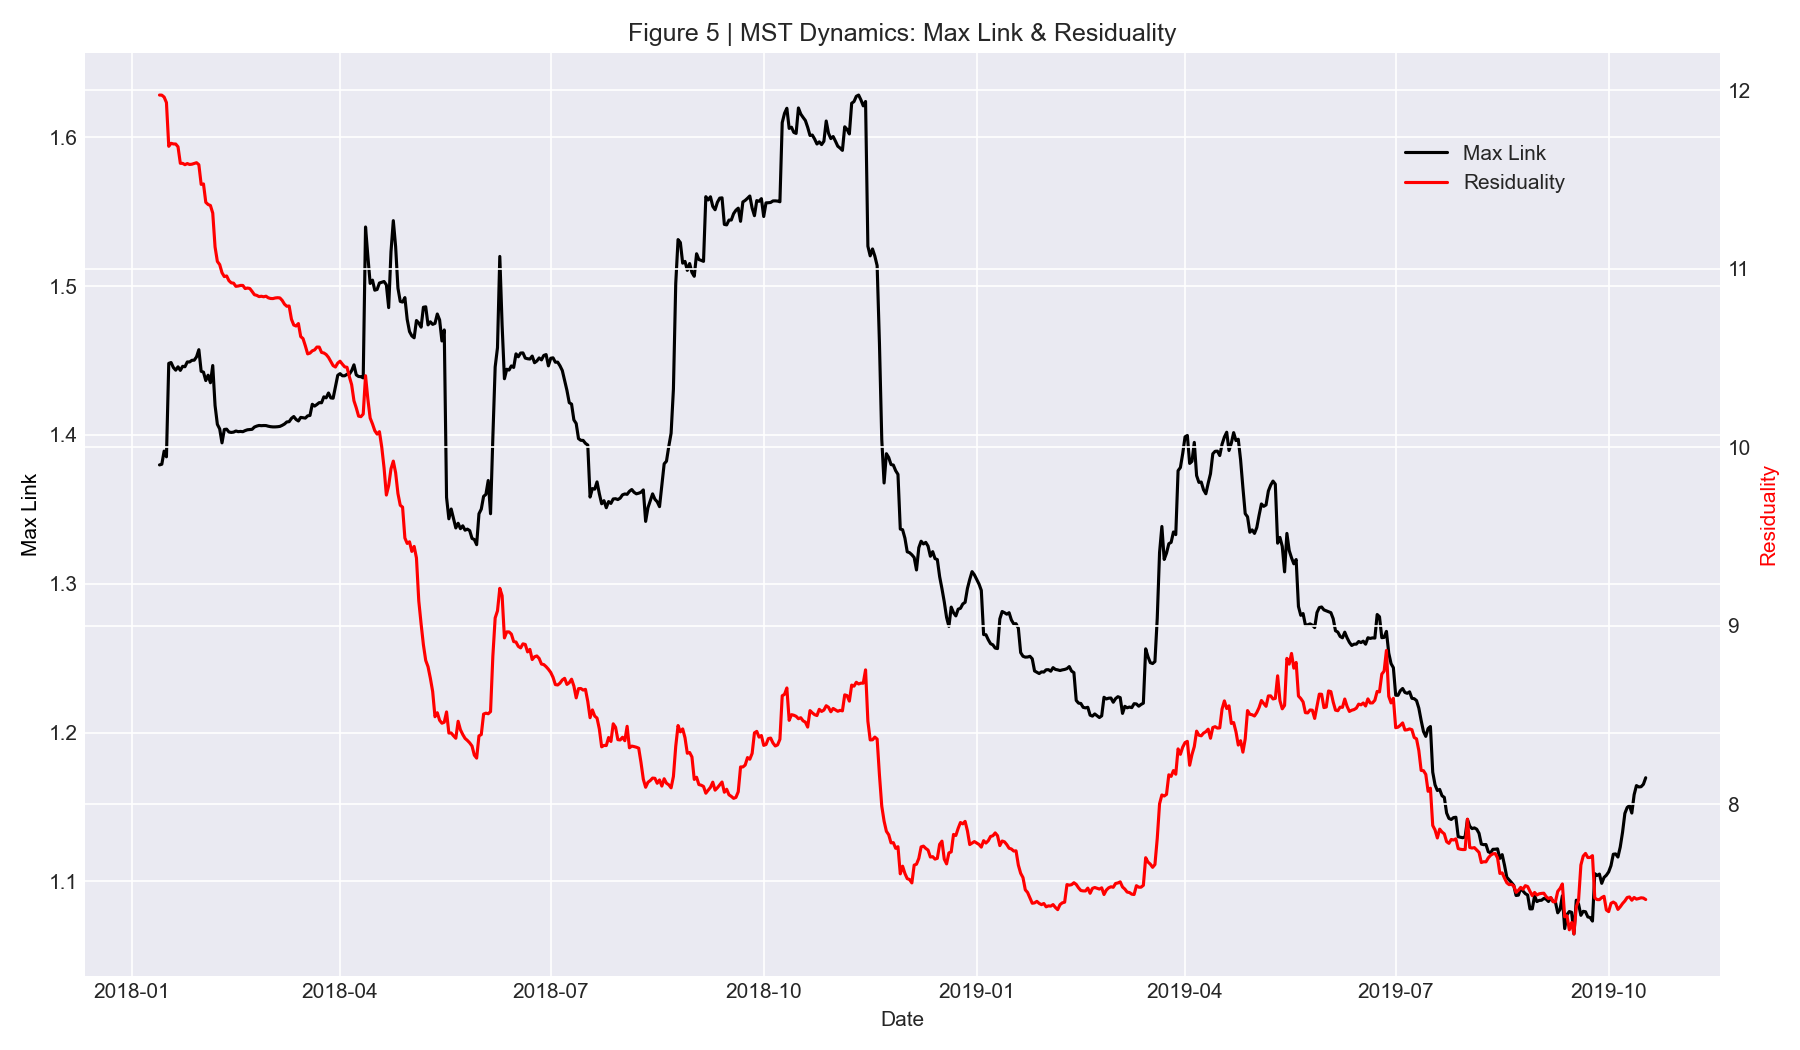
\includegraphics[width=0.8\textwidth]{figure_5_mst_dynamics.png}
    \caption{Dinamika MST: Ambang batas (\textit{max link}) dan koefisien \textit{residuality} sepanjang waktu.}
\end{figure}

%=============================================================================
\section{Sel 7 -- Implementasi Strategi Portofolio}
%=============================================================================
Setiap strategi diatur dalam kelas yang mewarisi \texttt{PortfolioStrategy}. Implementasi \textit{Network Markowitz} mencakup penalti sentralitas melalui parameter $\gamma$.

\begin{lstlisting}[caption={Kelas-kelas strategi portofolio}]
class PortfolioStrategy:
    def __init__(self, name):
        self.name = name
        self.weights_history = []
        self.returns_history = []
    def get_weights(self, returns_data): raise NotImplementedError

class EquallyWeighted(PortfolioStrategy):
    def get_weights(self, returns_data):
        n = returns_data.shape[1]; return np.ones(n) / n

class ClassicalMarkowitz(PortfolioStrategy):
    """Optimasi Mean-Variance tradisional (minimasi varians portofolio)."""
    def get_weights(self, returns_data):
        n_assets = returns_data.shape[1]
        mu       = returns_data.mean().values
        S        = returns_data.cov().values

        objective   = lambda w: w @ S @ w
        constraints = [
            {'type': 'eq',   'fun': lambda w: np.sum(w) - 1},
            {'type': 'ineq', 'fun': lambda w: w @ mu - mu.mean()}
        ]
        res = minimize(objective, np.ones(n_assets) / n_assets,
                       method='SLSQP', bounds=[(0, 1)] * n_assets,
                       constraints=constraints)
        return res.x if res.success else np.ones(n_assets) / n_assets

class GlassoMarkowitz(PortfolioStrategy):
    """Markowitz dengan matriks presisi yang diestimasi via Graphical Lasso."""
    def get_weights(self, returns_data):
        n_assets = returns_data.shape[1]
        mu       = returns_data.mean().values
        try:
            glasso    = GraphicalLassoCV()
            glasso.fit(returns_data.values); S = glasso.covariance_
        except Exception:
            S = returns_data.cov().values
        objective   = lambda w: w @ S @ w
        constraints = [
            {'type': 'eq',   'fun': lambda w: np.sum(w) - 1},
            {'type': 'ineq', 'fun': lambda w: w @ mu - mu.mean()}
        ]
        res = minimize(objective, np.ones(n_assets) / n_assets,
                       method='SLSQP', bounds=[(0, 1)] * n_assets,
                       constraints=constraints)
        return res.x if res.success else np.ones(n_assets) / n_assets

class NetworkMarkowitz(PortfolioStrategy):
    """Network Markowitz: RMT + MST + penalti sentralitas eigenvector."""
    def __init__(self, name="Network Markowitz", gamma=0):
        super().__init__(name); self.gamma = gamma
    def get_weights(self, returns_data):
        n_assets = returns_data.shape[1]
        mu       = returns_data.mean().values; sig = returns_data.std().values
        Cf = apply_rmt_filter(returns_data)
        dist = build_mst(Cf); cent = compute_eigenvector_centrality(dist)
        Sf = np.outer(sig, sig) * Cf
        objective   = lambda w: w @ Sf @ w + self.gamma * np.sum(cent * w)
        constraints = [
            {'type': 'eq',   'fun': lambda w: np.sum(w) - 1},
            {'type': 'ineq', 'fun': lambda w: w @ mu - mu.mean()}
        ]
        res = minimize(objective, np.ones(n_assets) / n_assets,
                       method='SLSQP', bounds=[(0, 1)] * n_assets,
                       constraints=constraints)
        return res.x if res.success else np.ones(n_assets) / n_assets

class GraphDiversification(PortfolioStrategy):
    """Strategi diversifikasi berbasis graf menggunakan Maximum Independent Set."""
    def __init__(self, name='Graph Diversification', corr_threshold=0.4):
        super().__init__(name); self.corr_threshold = corr_threshold
    def get_weights(self, r):
        n = r.shape[1]; assets = r.columns.tolist()
        sel = get_assets_graph_diversify(r, self.corr_threshold)
        w = np.zeros(n)
        if sel:
            for a in sel: w[assets.index(a)] = 1.0 / len(sel)
        else: w = np.ones(n) / n
        return w

class AdaptiveGraphPortfolio(PortfolioStrategy):
    """Adaptive Graph-Gated Portfolio (AGGP): Menggunakan Graph Density sebagai pemicu adaptif gamma."""
    def __init__(self, name="AGGP (Optimized)", sensitivity=2.0):
        super().__init__(name); self.sensitivity = sensitivity
    def get_weights(self, returns_data):
        n = returns_data.shape[1]; mu = returns_data.mean().values
        try:
            glasso = GraphicalLassoCV(cv=5); glasso.fit(returns_data.values)
            Sf = glasso.covariance_; Cf = glasso.correlation_
        except:
            Cf = apply_rmt_filter(returns_data)
            Sf = np.outer(returns_data.std(), returns_data.std()) * Cf
        adj = (np.abs(Cf) > 0.5).astype(int); G = nx.from_numpy_array(adj)
        density = nx.density(G); gamma_t = np.clip(density * self.sensitivity, 0.1, 0.9)
        dist = build_mst(Cf); cent = compute_eigenvector_centrality(dist)
        w_net = (1.0 / (cent + 1e-6)); w_net /= w_net.sum()
        res_mko = minimize(lambda w: w @ Sf @ w, np.ones(n)/n, method='SLSQP', 
                           bounds=[(0, 1)] * n, constraints=({'type': 'eq', 'fun': lambda x: np.sum(x) - 1}))
        return (1 - gamma_t) * res_mko.x + gamma_t * w_net
\end{lstlisting}

%=============================================================================
\section{Sel 8 -- Framework Backtesting}
%=============================================================================
Sistem pengujian menggunakan jendela bertahap (\textit{rolling window}) dengan biaya transaksi tetap sebesar 0.1\% (10 basis points) untuk merefleksikan kondisi perdagangan riil.

\begin{lstlisting}[caption={Fungsi simulasi backtest}]
def backtest_strategy(strategy, df_returns, window_size=120, rebalance_freq=7, transaction_cost=0.001):
    portfolio_returns = []; dates = []
    for i in range(window_size, len(df_returns), rebalance_freq):
        train = df_returns.iloc[i-window_size:i]
        w = strategy.get_weights(train)
        test_end = min(i + rebalance_freq, len(df_returns))
        test_data = df_returns.iloc[i:test_end]
        for j in range(len(test_data)):
            daily_ret = np.dot(w, test_data.iloc[j].values)
            if j == 0 and len(portfolio_returns) > 0:
                daily_ret -= transaction_cost
            portfolio_returns.append(daily_ret)
            dates.append(test_data.index[j])
    res_df = pd.DataFrame({'date': dates, 'return': portfolio_returns})
    res_df['cumulative_return'] = (1 + res_df['return']).cumprod()
    return {'strategy': strategy.name, 'returns': np.array(portfolio_returns),
            'cumulative_returns': res_df['cumulative_return'].values, 'results_df': res_df}
\end{lstlisting}

%=============================================================================
\section{Sel 9 -- Eksekusi Backtesting}
%=============================================================================
Setelah struktur strategi didefinisikan, dilakukan simulasi backtesting untuk semua varian strategi, termasuk benchmark CRIX dan model usulun dengan berbagai nilai penalti $\gamma$.

# --- Inisialisasi strategi ---
gamma_values = [0.005, 0.025, 0.05, 0.15, 0.7, 1.0]
strategies = [
    EquallyWeighted("EW"), ClassicalMarkowitz("CM"),
    GlassoMarkowitz("GM"), NetworkMarkowitz("NW (gamma=0)", gamma=0),
] + [NetworkMarkowitz(f"NW (gamma={g})", gamma=g) for g in gamma_values] + [
    GraphDiversification('Graph Divers. (theta=0.4)', corr_threshold=0.4),
    GraphDiversification('Graph Divers. (theta=0.5)', corr_threshold=0.5),
    RMTGraphDiversification('RMT GD (theta=0.4)',   corr_threshold=0.4),
    AdaptiveGraphPortfolio("AGGP (Optimized)", sensitivity=2.0)
]

# --- Eksekusi backtest ---
results = {}
for strat in strategies:
    results[strat.name] = backtest_strategy(strat, df_returns)
\end{lstlisting}

%=============================================================================
\section{Sel 10 -- Analisis Performa Periodik (Table 2)}
%=============================================================================
Bagian ini menghasilkan tabel perbandingan performa kumulatif yang disampel setiap 4 bulan (Januari, Mei, dan September), mereplikasi format pelaporan hasil pada paper acuan (Tabel 2).

\begin{table}[h]
    \centering
    \footnotesize
    \caption{TABLE 2 | Cumulative Profits and Losses (Struktur Output)}
    \begin{tabular}{lccccccccc}
        \toprule
        Period & CRIX & GM & EW & CM & NW & GD & RMT-GD & AGGP \\
        \midrule
        Jan-2018 & ... & ... & ... & ... & ... & ... & ... & ... \\
        May-2018 & ... & ... & ... & ... & ... & ... & ... & ... \\
        Sep-2018 & ... & ... & ... & ... & ... & ... & ... & ... \\
        \bottomrule
    \end{tabular}
\end{table}

\begin{lstlisting}[caption={Kalkulasi Profit/Loss Kumulatif Periodik (Jan, Mei, Sep)}]
target_dates = ['2018-01-31', '2018-05-31', '2018-09-30', 
                '2019-01-31', '2019-05-31', '2019-09-30']
table2_rows = []
for strat_name, res in results.items():
    df_res = res['results_df'].set_index('date')
    row = {'Strategy': strat_name}
    for td in target_dates:
        idx = df_res.index.searchsorted(pd.Timestamp(td))
        idx = min(idx, len(df_res) - 1)
        cum_ret = (df_res['cumulative_return'].iloc[idx] - 1) * 100
        row[td] = round(cum_ret, 2)
    table2_rows.append(row)
table2 = pd.DataFrame(table2_rows)
\end{lstlisting}

%=============================================================================
\section{Sel 11 -- Visualisasi Performa Kumulatif (Figure 6)}
%=============================================================================
Langkah terakhir adalah memvisualisikan pertumbuhan nilai portofolio. Sesuai dengan metodologi pada paper acuan, grafik ini menunjukkan evolusi nilai portofolio dengan asumsi investasi awal sebesar 100 USD.

\begin{lstlisting}[caption={Visualisasi Cumulative Returns (Scale 100 USD)}]
plt.figure(figsize=(14, 7))
for name, res in results.items():
    # Mengalikan cumulative_returns (basis 1.0) dengan 100 untuk skala USD
    plt.plot(res['results_df']['date'], res['cumulative_returns'] * 100, label=name)

plt.title('FIGURE 6 | Performances of different portfolio strategies')
plt.xlabel('Date'); plt.ylabel('Portfolio Value (USD)')
plt.legend(bbox_to_anchor=(1.02, 1), loc='upper left')
plt.grid(True, alpha=0.3); plt.show()
\end{lstlisting}

    \centering
    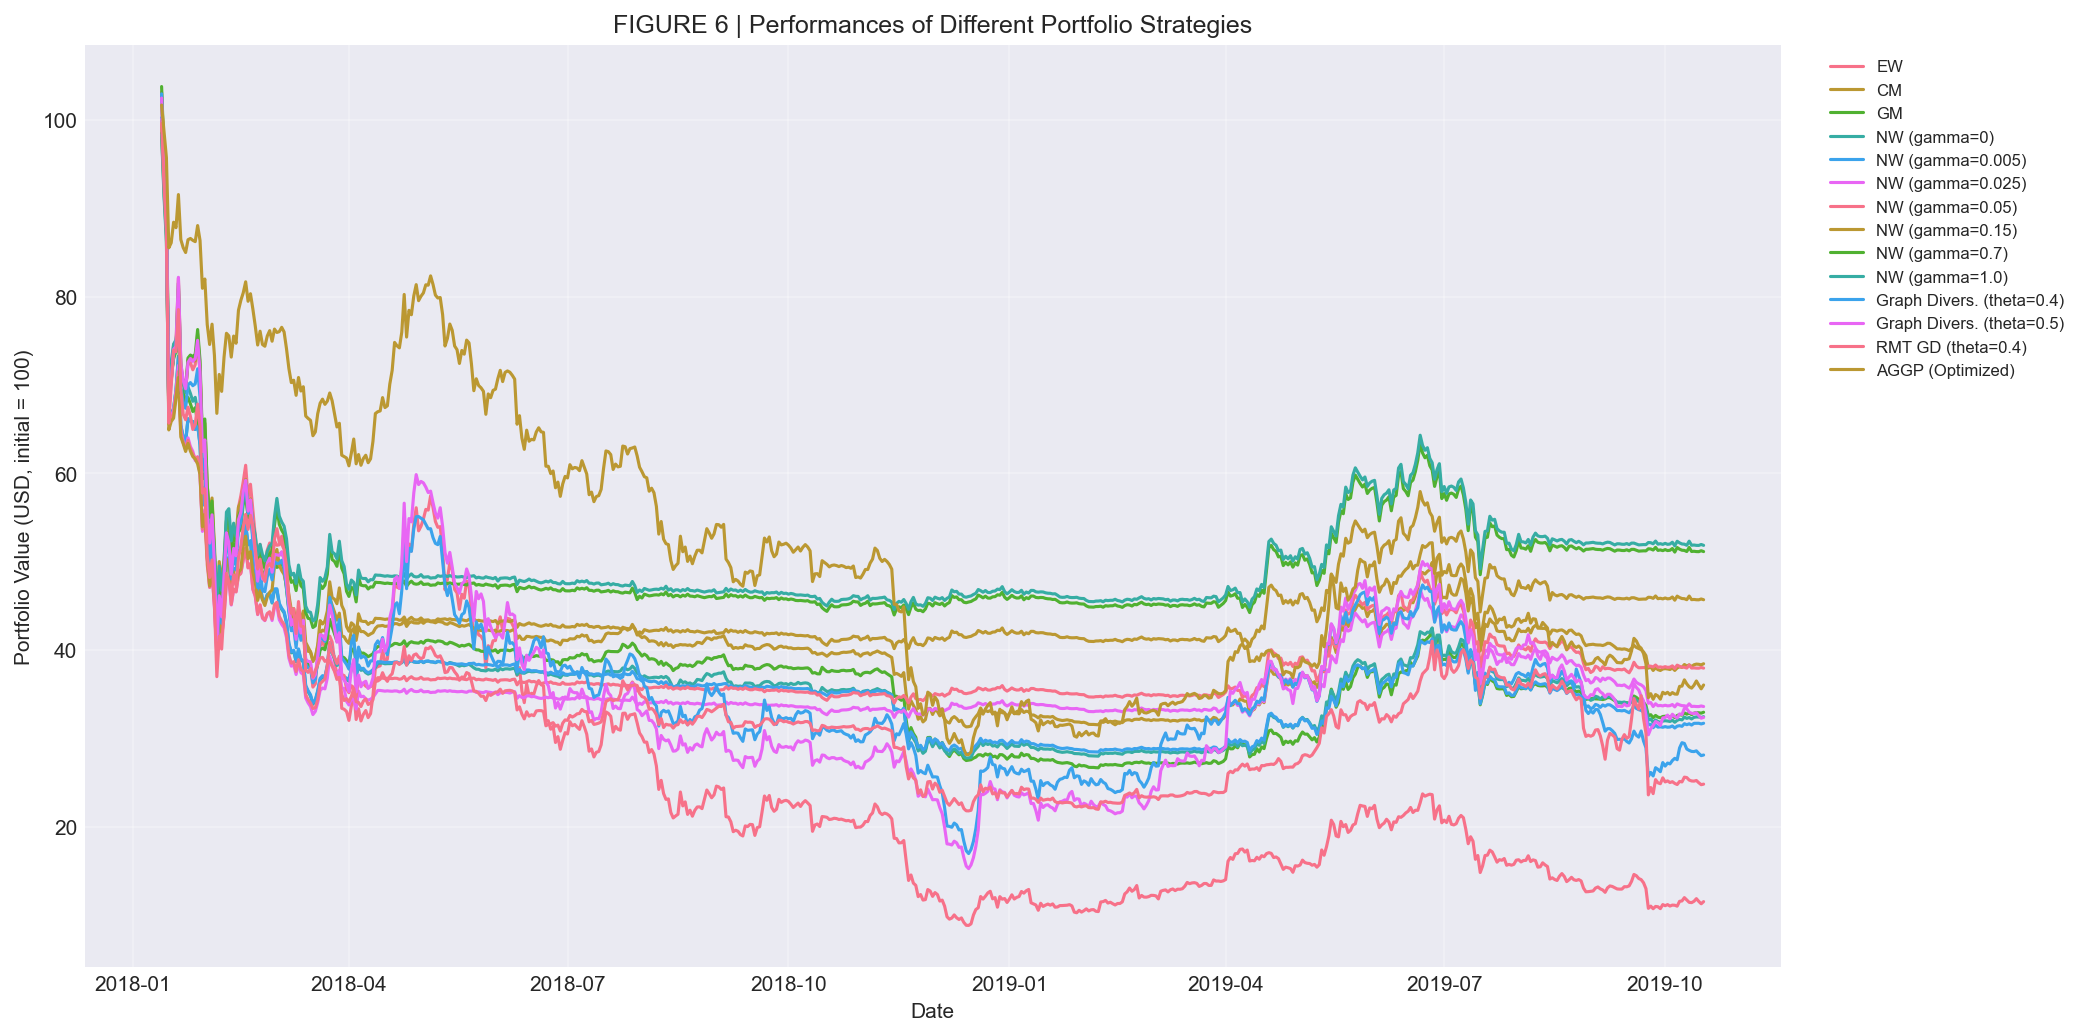
\includegraphics[width=1.0\textwidth]{cumulative_returns.png}
    \caption{\textbf{FIGURE 6 | Performances of different portfolio strategies.} The plot reports the profits and losses of a portfolio with initial value of 100 USD obtained by the CRIX benchmark index [Benchmark (CRIX)], the optimization using the Markowitz approach with the variance-covariance matrix filtered by Glasso (Glasso Markowitz), the naive portfolio (Equally Weighted), our optimization using RMT and MST applied to the variance-covariance matrix (Network Markowitz), our model based on different values of $\gamma$, the standard Markowitz portfolio (Classical Markowitz), and the proposed \textbf{Adaptive Graph-Gated Portfolio (AGGP)}. The portfolio values are plotted for the period 7 January 2018--17 October 2019.}
\end{figure}

%=============================================================================
\section{Sel 12 -- Analisis Risiko Periodik (Table 3)}
%=============================================================================
Selain return, risiko juga diukur secara periodik menggunakan \textit{Value at Risk} (VaR) dengan tingkat kepercayaan 95\%. Sesuai dengan paper acuan, nilai yang disajikan adalah nilai absolut dikalikan dengan faktor skala 100.

\begin{lstlisting}[caption={Kalkulasi VaR 95\% Periodik}]
# Menghitung VaR untuk jendela 4 bulan terakhir di setiap titik sampling
v = abs(calculate_var(returns_segment, 0.95)) * 100
\end{lstlisting}

\begin{table}[h]
    \centering
    \footnotesize
    \caption{\textbf{TABLE 3 | VaR.} This table shows the 4-months Value at Risk of portfolios under different strategies for a confidence interval of 95\%. In particular, the VaR is computed for CRIX, EW, NW, GM, CM, and the optimized \textbf{AGGP}. All values are expressed in absolute terms multiplied by a scale factor of 100.}
    \begin{tabular}{lcccccc}
        \toprule
        Period & CRIX & EW & NW & GM & CM & AGGP \\
        \midrule
        Jan-2018 & ... & ... & ... & ... & ... & ... \\
        May-2018 & ... & ... & ... & ... & ... & ... \\
        Sep-2018 & ... & ... & ... & ... & ... & ... \\
        \bottomrule
    \end{tabular}
\end{table}

%=============================================================================
\section{Sel 13 -- Analisis Risk-Adjusted Return (Table 4)}
%=============================================================================
Metrik terakhir yang dianalisis secara berkala adalah \textit{Sharpe ratio} untuk mengevaluasi imbal hasil yang disesuaikan dengan risiko.

\begin{lstlisting}[caption={Kalkulasi Sharpe Ratio Periodik}]
# Sharpe Ratio = Mean Return / Std Dev Return (jendela 4 bulan)
sr = np.mean(returns_segment) / np.std(returns_segment)
\end{lstlisting}

\begin{table}[h]
    \centering
    \footnotesize
    \caption{\textbf{TABLE 4 | Sharpe ratio.} This table shows the 4-months values of Sharpe ratio of portfolios under different strategies. In particular, the SR is computed for GM, EW, CM, NW, and the optimized \textbf{AGGP}.}
    \begin{tabular}{lcccccc}
        \toprule
        Period & GM & EW & CM & NW & $\gamma=0.15$ & AGGP \\
        \midrule
        Jan-2018 & ... & ... & ... & ... & ... & ... \\
        May-2018 & ... & ... & ... & ... & ... & ... \\
        Sep-2018 & ... & ... & ... & ... & ... & ... \\
        \bottomrule
    \end{tabular}
\end{table}

%=============================================================================
\section{Sel 14 -- Analisis Tail-Risk (Table 5)}
%=============================================================================
Metrik terakhir yang disajikan adalah \textit{Rachev ratio} (RR). RR memberikan wawasan tentang asimetri distribusi imbal hasil pada ekor (tails), yang sering ditemukan pada pasar kripto.

\begin{lstlisting}[caption={Kalkulasi Rachev Ratio Periodik}]
# Rachev Ratio = CVaR_upper (10%) / CVaR_lower (10%)
rr = calculate_rachev_ratio(returns_segment, alpha=0.10)
\end{lstlisting}

\begin{table}[h]
    \centering
    \footnotesize
    \caption{\textbf{TABLE 5 | Rachev ratio.} This table shows the 4-months values of Rachev Ratio (RR) of portfolios under different strategies. In particular, the RR is computed for GM, EW, CM, NW, and the proposed \textbf{AGGP}.}
    \begin{tabular}{lcccccc}
        \toprule
        Period & GM & EW & CM & NW & $\gamma=0.15$ & AGGP \\
        \midrule
        Jan-2018 & ... & ... & ... & ... & ... & ... \\
        May-2018 & ... & ... & ... & ... & ... & ... \\
        Sep-2018 & ... & ... & ... & ... & ... & ... \\
        \bottomrule
    \end{tabular}
\end{table}

%=============================================================================
\section{Sel 15 -- Analisis Fase Pasar (Market Phase Analysis Mapping)}
%=============================================================================
Untuk menguji kekokohan strategi di berbagai kondisi pasar, dilakukan pemetaan performa ke dalam tiga fase utama: \textbf{Bearish} (Januari 2018 -- Maret 2019), \textbf{Recovery} (April 2019 -- Juni 2019), dan \textbf{Stable/Sideways} (Juli 2019 -- Oktober 2019). Hal ini ditujukan untuk membuktikan bahwa model \textbf{AGGP} mampu beradaptasi sebagai \textit{"All-Terrain Model"} yang tangguh saat pasar tertekan (\textit{Bearish}) berkat komponen Glasso/GM, dan agresif memanfaatkan peluang saat pasar pulih (\textit{Recovery}) berkat komponen Network (NW).

\begin{lstlisting}[caption={Kalkulasi Metrik Berdasarkan Fase Pasar}]
# Definisi Fase Pasar
fase_pasar = {
    'Bearish': ('2018-01-01', '2019-03-31'),
    'Recovery': ('2019-04-01', '2019-06-30'),
    'Stable': ('2019-07-01', '2019-10-17')
}

# (Kode implementasi kalkulasi Sharpe dan Rachev Ratio untuk tiap fase)
\end{lstlisting}

\begin{table}[h]
    \centering
    \footnotesize
    \caption{\textbf{TABLE 6 | Market Phase Performance.} Perbandingan \textit{Sharpe Ratio} dan \textit{Rachev Ratio} untuk setiap model pada tiga kondisi pasar yang berbeda.}
    \begin{tabular}{lcccccc}
        \toprule
        Market Phase & EW & CM & GM & NW & $\gamma=0.15$ & AGGP \\
        \midrule
        \multicolumn{7}{c}{\textit{Panel A: Sharpe Ratio}} \\
        Bearish & ... & ... & ... & ... & ... & ... \\
        Recovery & ... & ... & ... & ... & ... & ... \\
        Stable & ... & ... & ... & ... & ... & ... \\
        \midrule
        \multicolumn{7}{c}{\textit{Panel B: Rachev Ratio ($\alpha=10\%$)}} \\
        Bearish & ... & ... & ... & ... & ... & ... \\
        Recovery & ... & ... & ... & ... & ... & ... \\
        Stable & ... & ... & ... & ... & ... & ... \\
        \bottomrule
    \end{tabular}
\end{table}

\end{document}
